%%%%%%%%%%%%%%%%%%%%%%%%%%%%%%%%%%%%%%%%%
% University Assignment Title Page 
% LaTeX Template
% Version 1.0 (27/12/12)
%
% This template has been downloaded from:
% http://www.LaTeXTemplates.com
%
% Original author:
% WikiBooks (http://en.wikibooks.org/wiki/LaTeX/Title_Creation)
%
% License:
% CC BY-NC-SA 3.0 (http://creativecommons.org/licenses/by-nc-sa/3.0/)
% 
% Instructions for using this template:
% This title page is capable of being compiled as is. This is not useful for 
% including it in another document. To do this, you have two options: 
%
% 1) Copy/paste everything between \begin{document} and \end{document} 
% starting at \begin{titlepage} and paste this into another LaTeX file where you 
% want your title page.
% OR
% 2) Remove everything outside the \begin{titlepage} and \end{titlepage} and 
% move this file to the same directory as the LaTeX file you wish to add it to. 
% Then add \input{./title_page_1.tex} to your LaTeX file where you want your
% title page.
%
%%%%%%%%%%%%%%%%%%%%%%%%%%%%%%%%%%%%%%%%%
%\title{Title page with logo}
%----------------------------------------------------------------------------------------
%	PACKAGES AND OTHER DOCUMENT CONFIGURATIONS
%----------------------------------------------------------------------------------------

\documentclass[12pt]{article}
\usepackage{wrapfig}
\usepackage[english]{babel}
\usepackage[utf8]{inputenc}
\usepackage{amsmath}
\usepackage{graphicx}
\usepackage[colorinlistoftodos]{todonotes}

\begin{document}

\begin{titlepage}

\newcommand{\HRule}{\rule{\linewidth}{0.5mm}} % Defines a new command for the horizontal lines, change thickness here

\center % Center everything on the page
 
%----------------------------------------------------------------------------------------
%	HEADING SECTIONS
%----------------------------------------------------------------------------------------

\textsc{\LARGE Universidad de Sonora }\\[0.3cm] % Name of your university/college
\textsc{\Large Departamento de Ciencias Naturales y Exactas  }\\[0.3cm]
\textsc{\Large Licenciatura en Física }\\[0.3cm]
\textsc{\Large Física computacional I}\\[0.3cm] % Major heading such as course name
 % Minor heading such as course title

%----------------------------------------------------------------------------------------
%	TITLE SECTION
%----------------------------------------------------------------------------------------

\HRule \\[0.1cm]
{ \huge \bfseries Actividad 6\\  Sistema de Resortes Acoplados}\\[0.01cm] % Title of your document
\HRule \\[1.5cm]

 
%----------------------------------------------------------------------------------------
%	AUTHOR SECTION
%----------------------------------------------------------------------------------------

\begin{minipage}{0.4\textwidth}
\begin{flushleft} \large
\emph{Alumno:}\\
Gómez García \\Manuel Ignacio\\ %Grupo 1 % Your name
\end{flushleft}
\end{minipage}
~
\begin{minipage}{0.4\textwidth}
\begin{flushright} \large
\emph{Profesor:} \\
Lizarraga Celaya\\Carlos\\%Dept. of CSE % Supervisor's Name
\end{flushright}
\end{minipage}\\[1cm]

% If you don't want a supervisor, uncomment the two lines below and remove the section above
%\Large \emph{Author:}\\
%John \textsc{Smith}\\[3cm] % Your name

%----------------------------------------------------------------------------------------
%	DATE SECTION
%----------------------------------------------------------------------------------------

{\large \date[25 de mayo, 2018 \\Hermosillo, Sonora}\\[1cm] % Date, change the \today to a set date if you want to be precise

%----------------------------------------------------------------------------------------
%	LOGO SECTION
%----------------------------------------------------------------------------------------


\includegraphics[height=5.5cm]{Logo}\\[0.5cm] % Include a department/university logo - this will require the graphicx package
 
%----------------------------------------------------------------------------------------

\vfill % Fill the rest of the page with whitespace

\end{titlepage}


%\begin{abstract}
%Your abstract.
%\end{abstract}
\begin{titlepage}
\title {Jupyter not\ebook}
\end{titlepage}

\section{Introducción}

En esta práctica nos enfocaremos en las Ecuaciones Diferenciales Ordinarias pues existen una gran variedad de técnicas a emplear para encontrar una solución. En particular, las ecuaciones no lineales debido a la gran cantidad y poder de algoritmos existentes además de la mínima potencia gráfica que requieren los sistemas de álgebra computacional, como lo son $Mathematica$ y $Maple$.

El ejemplo que utilizaremos será el clásico ejercicio de dos masas y dos resortes para armar el sistema que se encuentra colgando del techo. El problema presenta de forma natural ya una Ecuación Diferencial de Segundo Orden. Al diferenciar y sustituir una ecuación en otra podemos obtener una Ecuación Diferencial de Cuarto Orden, haciendo esto que el problema se vuelva interesante puesto que usualmente en la física son de Segundo Orden todas las E.D. que suelen surgir.

La forma en que ahora se nos presenta el ejercicio nos permite explorar aún más fenómenos involucrados en nuestro sistema, siendo estos más interesante al agregar ciertos factores que involucran una oscilación forzada.

\section{Modelo de resortes acoplados}

\begin{figure}[h!]
	\begin{center}
	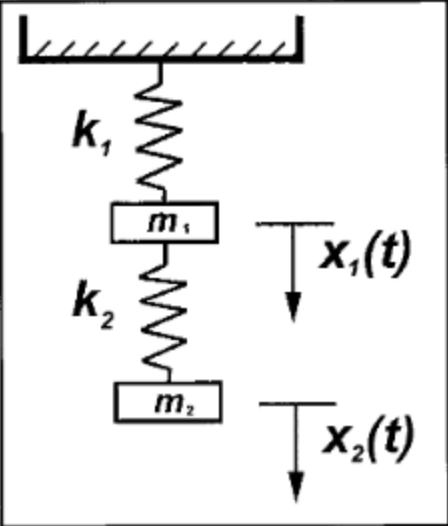
\includegraphics[height=6cm]{SistRes}
    \caption{Sistema de resortes acoplados}
	\end{center}
\end{figure}

\noindent Nuestro sistema a trabajar será como el mostrado en la figura 1. Los datos a recopilar serán primeramente las posiciones de cada una de las masas en las cuales alcanzan el equilibrio, siendo medidas desde su centro de masa hasta dicho punto donde el sistema se encuentra en reposo, de esta manera para $x_1(t)$ y $x_2(t)$. \\

\begin{center}
	\textbf{ASUMIENDO LA LEY DE HOOKE}
\end{center}


\noindent Si consideramos pequeñas oscilaciones, las fuerzas de restitución son de la forma $-k_1l_1$ y $-k_2l_2$ donde $l_1$ y $l_2$ son la elongación  o comprensión de cada resorte. El resorte superior al estar conectado a ambos percibe dos fuerzas distintas; el primer resorte que jala el bloque hacía arriba con una fuerza dada por $-k_1x_1$ y el segundo, que aplica una fuerza que se resiste a ser estirado, la cual es $-k(x_2-x_1)$. Si despreciamos el amortiguamiento, las ecuaciones de Newton para cada masa serían:

\begin{center}
$m_1a_1 = -k_1x_1 - k_2(x_1 - x_2)$ 
\\ \hspace{12 cm} (2.1)
\\ $m_2a_2 = -k_2(x_2 - x_1)$
\end{center}

De aquí, tenemos ahora dos E.D. de Segundo Orden entonces lo siguiente es encontrar una ecuación para $x_1$ sin involucrar a $x_2$, resolvemos la primer ecuación para $x_2$, que sería:

\begin{center}
	$x_2 = \frac{m_1a_1}{k_2} + \frac{k_1 + k_2}{k_2}x_1$
\end{center}

Ahora sustituimos el valor de $x_2$ en la segunda ecuación de (2.1), donde tenemos $m_2$, de modo que la sustitución resulta en lo siguiente:

\begin{center}
	$m_1m_2x_1^{(4)} + (m_2k_1 + k_2(m_1 + m_2))a_1 + k_1k_2x_1  = 0$
\end{center}

Dando por resultado que el movimiento de $m_1$ esta dado por una E.D. de Cuarto Grado. 

Bien, lo siguiente será despejar a $x_1$ para encontrar una E.D. en términos de $x_2$ y tenemos que:

\begin{center}
	$x_1 = \frac{m_2}{k_2}a_2 + x_2$
\end{center}

Tras sustituir en la primer ecuación de (2.1) el valor obtenido de $x_1$, tendremos:

\begin{center}
	$m_1m_2x_2^{(4)} + (m_2k_1 + k_2(m_1 + m_2))a_2 + k_1k_2x_2 = 0$
\end{center}

Como podemos ver, resulta que ambas E.D. se rigen bajo el mismo comportamiento, siendo la única diferencia la posición de cada una de las masas.
Como es costumbre, podríamos tomar los valores iniciales de ambas posiciones y velocidades como 0, de modo que para resolver el problema será necesario solucionar dos problemas de valor inicial de Cuarto Orden. \\

\begin{center}
	\textbf{EJEMPLOS CON LA MISMA MASA}
\end{center}

\noindent Si hacemos que ambos cuerpos posean la misma masa, $m_1 = m_2 = 1$. Y en el caso de que no existe amortiguamiento o una fuerza externa, la ecuación para el movimiento termina siendo:

\begin{center}
	$m^{4} + (k_1 + 2k_2)m^{2} + k_1k_2 = 0$
\end{center}

Y esta ecuación anterior tiene como raíces:

\begin{center}
	$\pm \sqrt[]{-\frac{1}{2}k_1 + k_2 \pm\frac{1}{2}\sqrt[]{k_1^{2} + 4k_2^{2}} }$
\end{center}

\paragraph{\textbf{Ejemplo 2.1}}
Describiremos el movimiento para el sistema de resortes acoplados con los siguientes valores: $k_1 = 6$, $k_2 = 4$, $x_1 = 1$, $x_2 = 2$, $v_1 = 0$ \& $v_2 = 0$.

Podemos ver que las raíces de la ecuación característica serían $\pm\sqrt[]{2}i$ y $\pm2\sqrt[]{3}i$. Con ello obtendremos una ecuación general que sería:

\begin{center}
	$x(t) = c_1 Cos \sqrt[]{2} t + c_2 Sen \sqrt[]{2} t + c_3 cos 2\sqrt[]{3}t + c_4 sen2\sqrt[]{3}t$
\end{center}

En conjunto con las ecuaciones anteriores y esta última llegaremos a que la solución para $x_1$ \& $x_2$ son:

\begin{center}
	$x_1(t) = cos \sqrt[]{2}t$
    \\ $x_2(t) = 2 cos \sqrt[]{2}t$
\end{center}

\vspace{3cm}

\paragraph{\textbf{Ejemplo 2.2}}
En este ejemplo, las constantes $k_1$, $k_2$, $v_1$ \& $v_2$ mantienen los valor anterior mientras que $x_1 = -2$ \& $x_2 = 1$.
Dando ahora como resultado:

\begin{center}
	$x_1(t) = -2 Cos 2 \sqrt[]{3} t$
    \\ $x_2(t) = Cos 2 \sqrt[]{3} t$
\end{center}

\paragraph{\textbf{Ejemplo 2.3}}
Las valores para las constantes del resorte serán $k_1 = 0.4$ \& $k_2 = 1.808$, los de posición $x_1 = 0.5$ \& $x_2 = -0.5$, mientras que los de velocidad $v_1 = 0$ \& $v_2 = 0.7$. \\

\begin{center}
	\textbf{AMORTIGUAMIENTO}
\end{center}

\noindent El amortiguamiento usualmente encontrado es el de sustancias viscosas; en dichos casos el amortiguamiento es proporcional a la velocidad. El amortiguamiento de cada masa es independiente al de la otra, por lo cual ahora hemos de expresar sus ecuaciones de movimiento añadiendo el siguiente término $-\delta_n a_n$, de modo que si suponemos que los coeficientes $\delta_n$  son pequeños, las ecuaciones se reescriben de la siguiente forma:

\begin{center}
	$ m_1a_1 = -\delta_1v_1-k_1x_1-k_2(x_1-x_2) $ \\
    $ m_2a_2 = -\delta_2v_2-k_2(x_2-x_1) $
\end{center}

Para obtener las ecuaciones que describen el movimiento de $x_1$ \& $x_2$ debemos despejar una de estas incógnitas de la ecuación y sustituir dicha expresión obtenida en la otra ecuación. De tal forma obtenemos para $x_1$ \& $x_2$, respectivamente:

\begin{center}
	$m_1m_2x_1^{(4)}+(m_1\delta_1+m_2\delta_2)x_1^{(3)}+(m_2k_1+k_2(m_1+m_2)+\delta_1\delta_2)a_1+(k_1\delta_2+k_2(\delta_1+\delta_2))v_1+k_1k_2x_1=0$ 
    
    \vspace{0.5cm}
    
    $m_1m_2x_2^{(4)}+(m_1\delta_1+m_2\delta_2)x_2^{(3)}+(m_2k_1+k_2(m_1+m_2)+\delta_1\delta_2)a_2+(k_1\delta_2+k_2(\delta_1+\delta_2))v_2+k_1k_2x_2=0$
\end{center}

Como podemos ver, las ecuaciones que describen el movimiento de ambos cuerpos son ecuaciones diferenciales lineales. \\

\textbf{Ejemplo 2.4} Asumiendo que $m_1=m_2=1$, $k_1=0.4$, $k_2=1.808$, $\delta_1=0.1$, $\delta_2=0.2$, $x_1=1$, $x_2=2$ \& $v_1=v_2=0.5$ describa el movimiento de las masas correspondientes.

\section{Creando el Sistema de Ecuaciones Diferenciales Ordinarias}

A lo largo de esta sección mostraremos el código utilizado para llevar a cabo los ejemplos 2.1, 2.2, 2.3 \& 2.4 que fueron planteados anteriormente.

Para comenzar, debemos definir un arreglo/vector que almacene los datos a utilizar, esto se debe hacer en los 4 códigos que veremos. Este es el bloque de código empleado.

\begin{figure}[h!]
	\begin{center}
		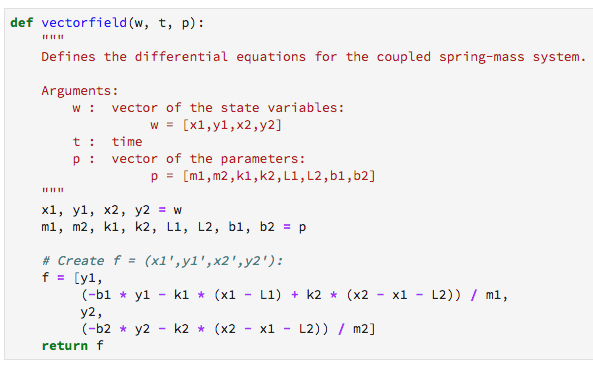
\includegraphics[width=10cm]{Ejem-Vec}
    	\caption{Arreglo que almacena los datos calculados.}
	\end{center}
\end{figure}

El siguiente bloque de código en los programas corresponde a los valores que definiremos (masa, coeficiente de restitución, posiciones y velocidades iniciales, entre otros más).

Para el \textbf{ejemplo 2.1}, el código usado se muestra en la \textbf{Figura \ref{Ejem2.1-Para}}, para el \textbf{ejemplo 2.2} la \textbf{Figura \ref{Ejem2.2-Para}}, para el \textbf{ejemplo 2.3} la \textbf{Figura \ref{Ejem2.3-Para}} y por último, tenemos la \textbf{Figura \ref{Ejem2.4-Para}} para el \textbf{ejemplo 2.4}.

\begin{figure}
	\begin{center}
		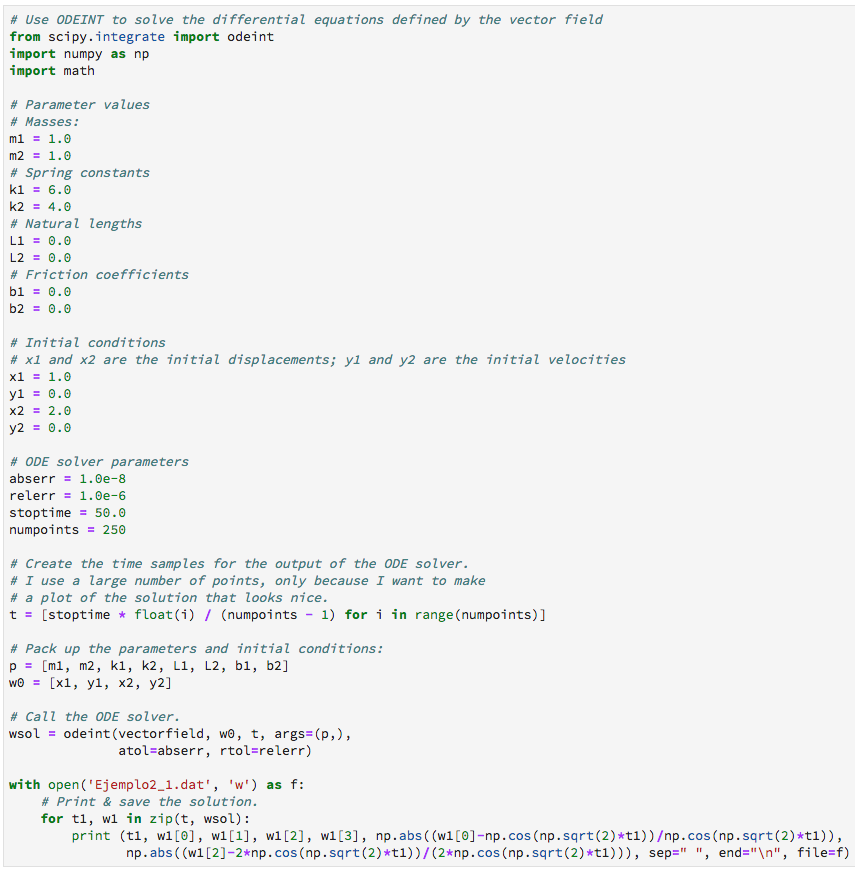
\includegraphics[height=17cm]{Ejem2_1-Para}
        \caption{Parámetros para el ejemplo 2.1}
        \label{Ejem2.1-Para}
    \end{center}
\end{figure}

\begin{figure}
	\begin{center}
        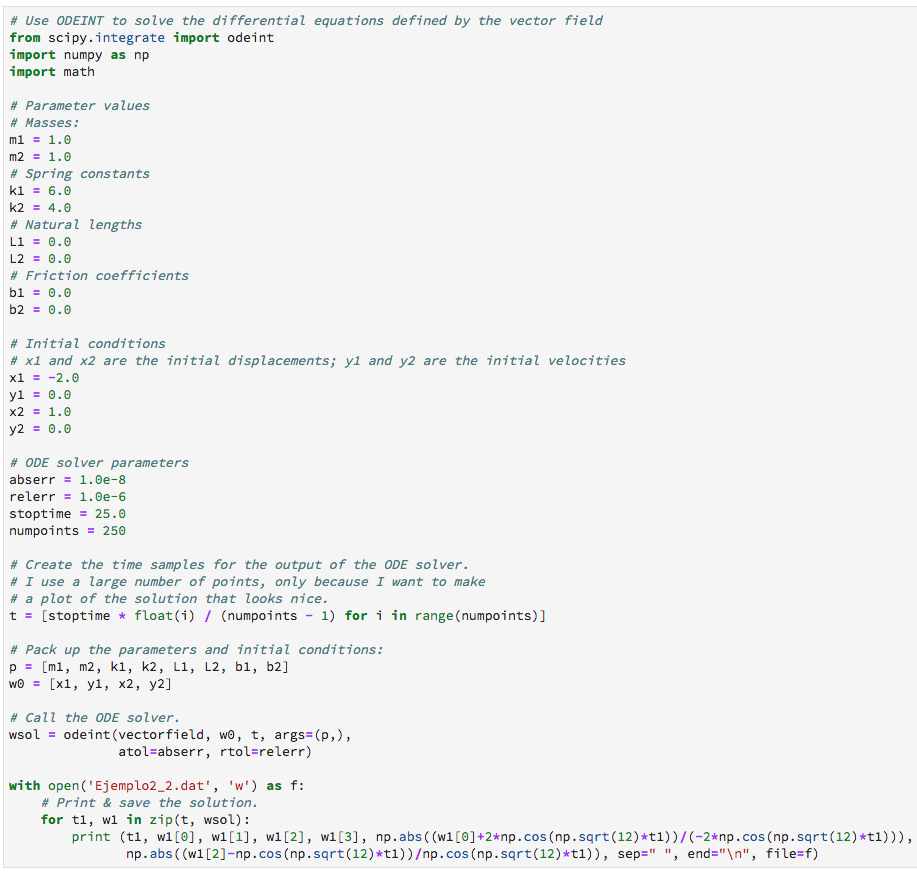
\includegraphics[height=16cm]{Ejem2_2-Para}
        \caption{Parámetros del ejemplo 2.2}
        \label{Ejem2.2-Para}
    \end{center}
\end{figure}
        
\begin{figure}
	\begin{center}
        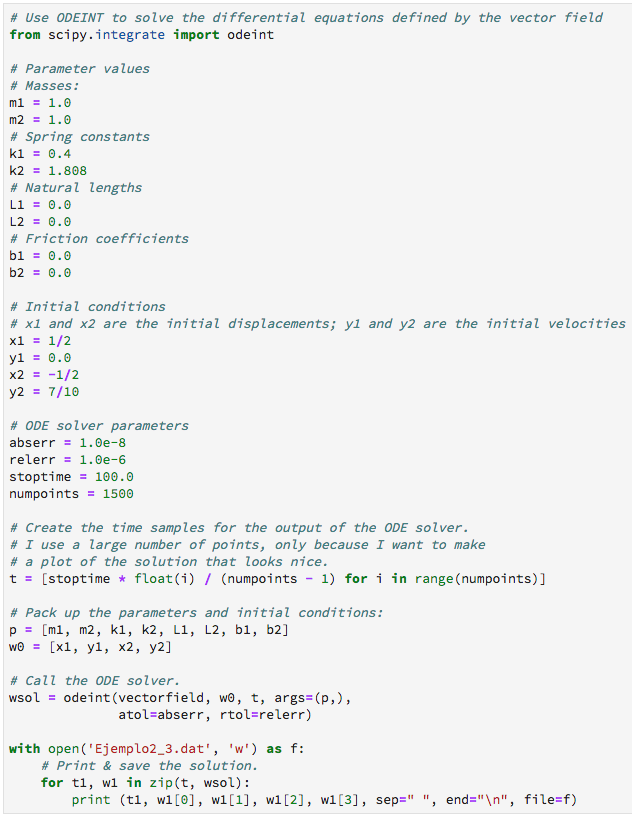
\includegraphics[height=17.5cm]{Ejem2_3-Para}
        \caption{Parámetros del ejemplo 2.3}
        \label{Ejem2.3-Para}
    \end{center}
\end{figure}
        
\begin{figure}
	\begin{center}
        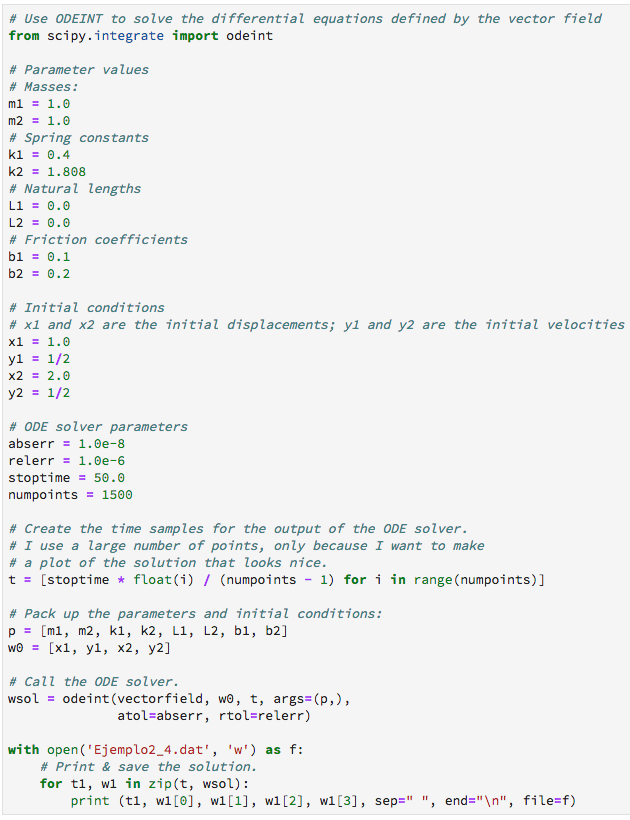
\includegraphics[height=17.5cm]{Ejem2_4-Para}
        \caption{Parámetros del ejemplo 2.4}
        \label{Ejem2.4-Para}
    \end{center}
\end{figure}

Lo siguiente consiste en escribir el código para generar cada una de las gráficas correspondientes. Para las gráficas del primer ejemplo usamos el código de la Figura \ref{Ejem2.1-CodA}. En dicho código vemos que se cargan primeramente las librerías que usaremos (esto se hace sólo una vez), después leeremos los datos desde el archivo que los contiene, especificándole a qué variable corresponde cada una de las series de datos, seguido de ello se hacen ajustes del gráfico -Nombre de los márgenes, grosor de las líneas, forma de visualizar, límites de los ejes, datos a gráficar-, y por último, guardamos nuestro archivo con el nombre que deseemos.

\noindent \textbf{NOTA:} Para el ejemplo 2.3 y 2.4, debemos omitir $e1$ y $e2$ de la lectura de datos.

\begin{figure}[h!]
	\begin{center}
        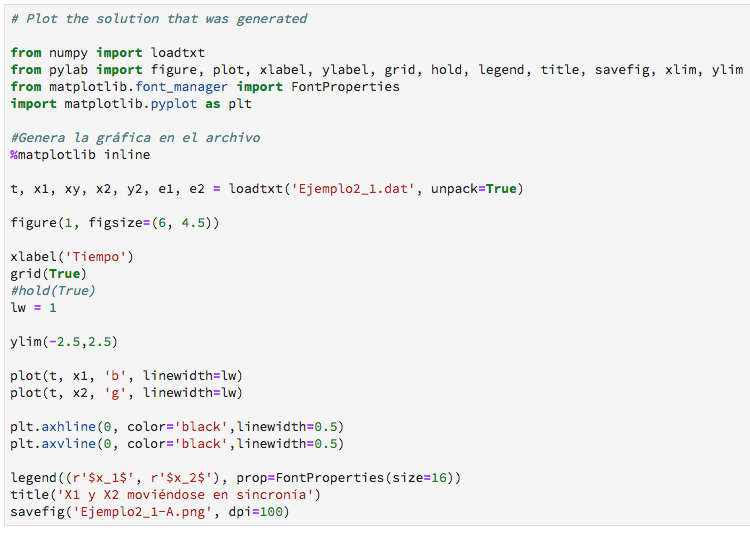
\includegraphics[height=10cm]{Ejem2_1-CodA}
        \caption{Código para la primer gráfica del ejemplo 2.1}
        \label{Ejem2.1-CodA}
    \end{center}
\end{figure}
        
\begin{figure}[h!]
	\begin{center}
        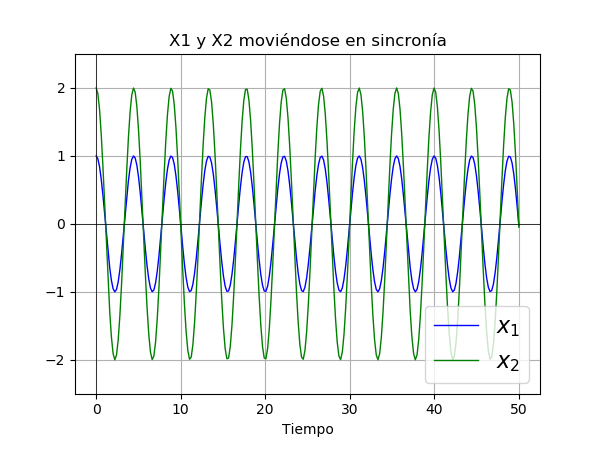
\includegraphics[height=8cm]{Ejem2_1-GrafA}
        \caption{Primer gráfica del ejemplo 2.1}
        \label{Ejem2.1-GrafA}
    \end{center}
\end{figure}

\begin{figure}[h!]
	\begin{center}
        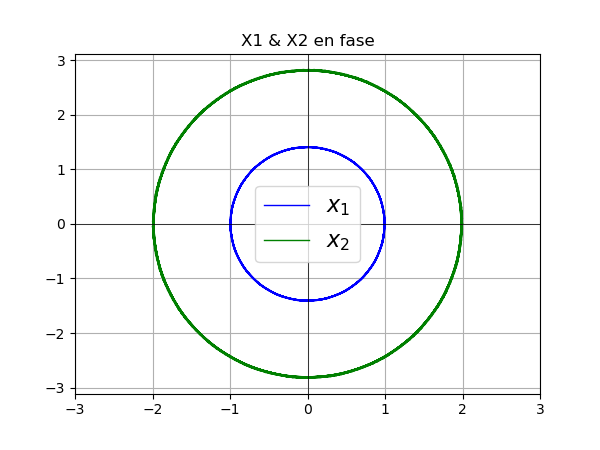
\includegraphics[height=9cm]{Ejem2_1-GrafB}
        \caption{Gráfica del ejemplo 2.1}

        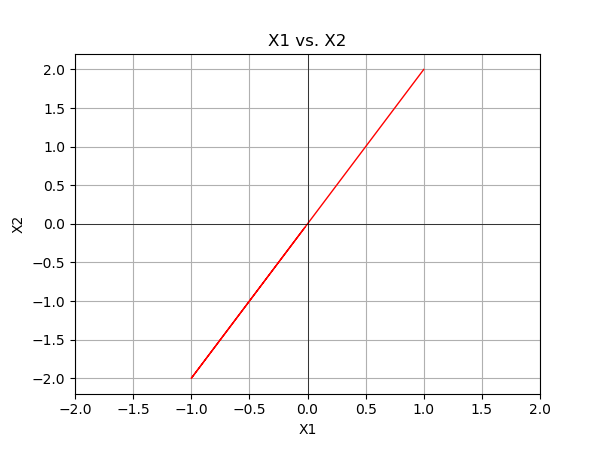
\includegraphics[height=9cm]{Ejem2_1-GrafC}
        \caption{Gráfica del ejemplo 2.1}
    \end{center}
\end{figure}

\begin{figure}[h!]
	\begin{center}
        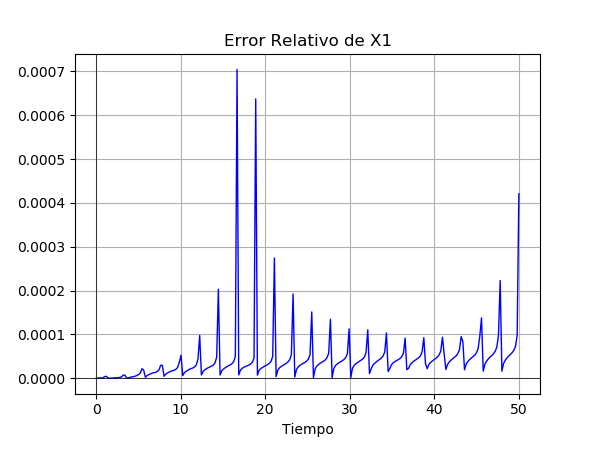
\includegraphics[height=9cm]{Ejem2_1-GrafErr1}
        \caption{Gráfica del ejemplo 2.1}

        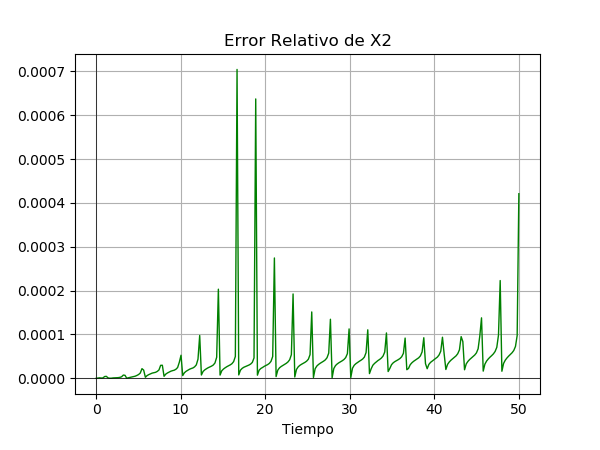
\includegraphics[height=9cm]{Ejem2_1-GrafErr2}
        \caption{Gráfica del ejemplo 2.1}
    \end{center}
\end{figure}

Ahora en base al tipo de gráfico que estemos por realizar habrá que variar los datos mencionados.

\bigskip

Por ejemplo, para las gráficas correspondientes al \textbf{ejemplo 2.2} van de la Figura \ref{Ejem2.2-GrafA} a la \ref{Ejem2.2-GrafErr2}, cambiamos los parámetros a los mencionados anteriormente y listo.

\vfill
\vline
\space
\par \vspace{1cm}

\begin{figure}[h!]
	\begin{center}
        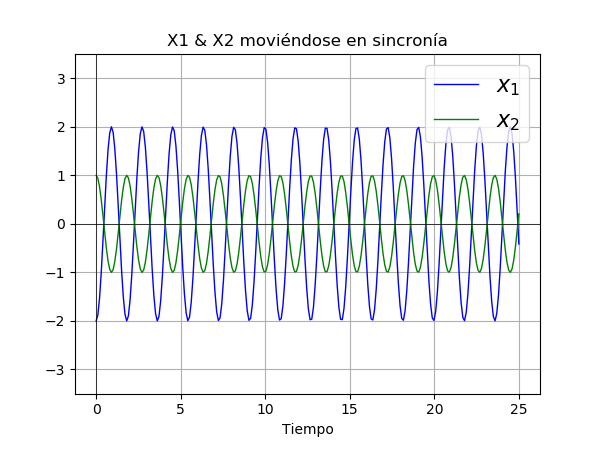
\includegraphics[height=9cm]{Ejem2_2-GrafA}
        \caption{Gráfica del ejemplo 2.2}
        \label{Ejem2.2-GrafA}

        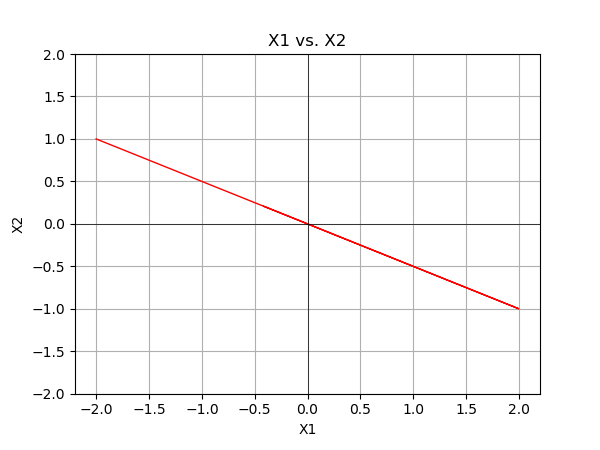
\includegraphics[height=9cm]{Ejem2_2-GrafB}
        \caption{Gráfica del ejemplo 2.2}
    \end{center}
\end{figure}

\begin{figure}[h!]
	\begin{center}
        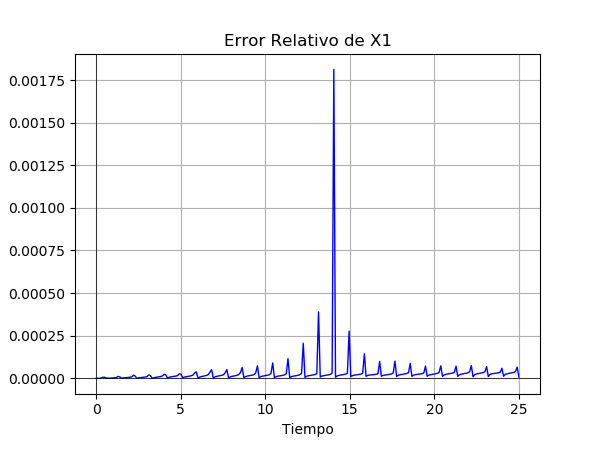
\includegraphics[height=9cm]{Ejem2_2-GrafErr1}
        \caption{Gráfica del ejemplo 2.2}

        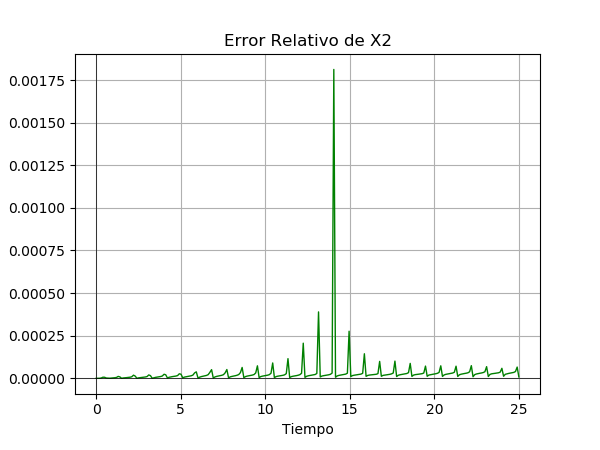
\includegraphics[height=9cm]{Ejem2_2-GrafErr2}
        \caption{Gráfica del ejemplo 2.2}
        \label{Ejem2.2-GrafErr2}
    \end{center}
\end{figure}

Para el \textbf{ejemplo 2.3}, de la Figura \ref{Ejem2.3-GrafA} a la \ref{Ejem2.3-GrafF}.

\begin{figure}[h!]
	\begin{center}
        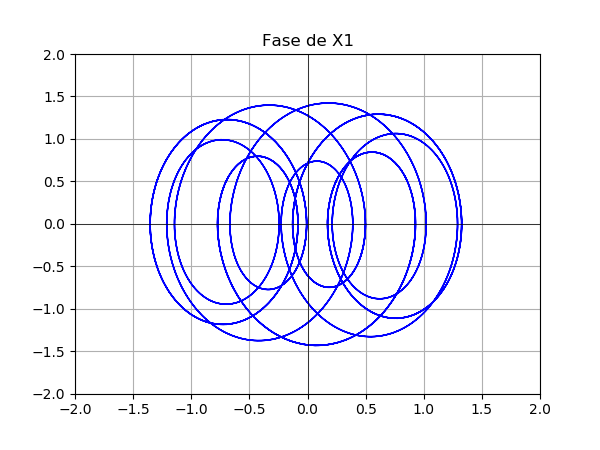
\includegraphics[height=9cm]{Ejem2_3-GrafA}
        \caption{Gráfica del ejemplo 2.3}
        \label{Ejem2.3-GrafA}

    	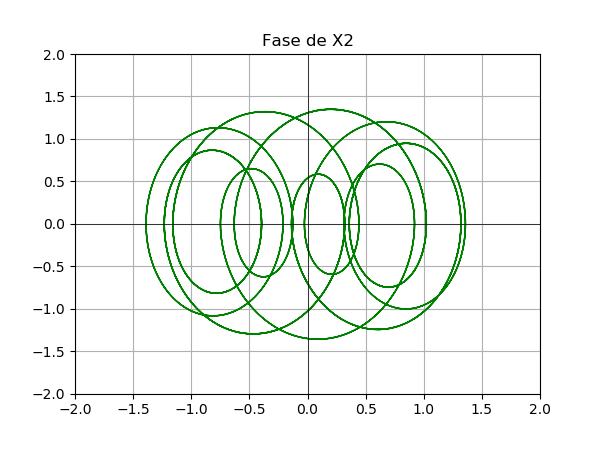
\includegraphics[height=9cm]{Ejem2_3-GrafB}
        \caption{Gráfica del ejemplo 2.3}
    \end{center}
\end{figure}

\begin{figure}[h!]
	\begin{center}
        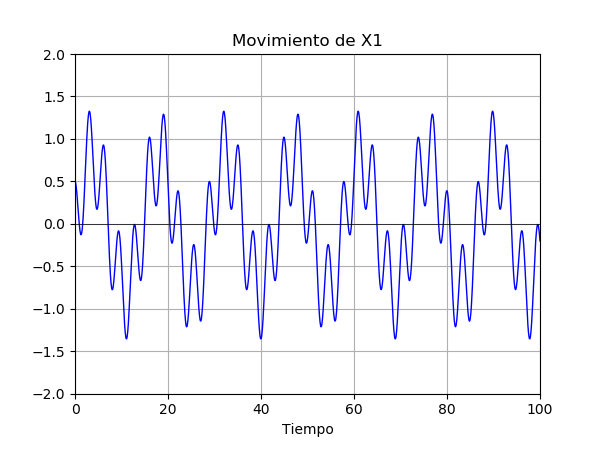
\includegraphics[height=9cm]{Ejem2_3-GrafC}
        \caption{Gráfica del ejemplo 2.3}

        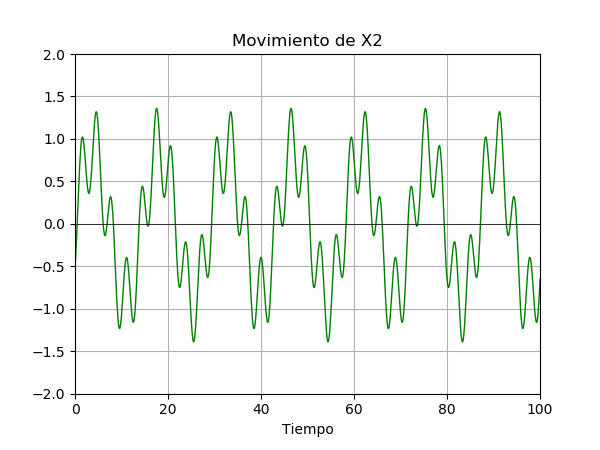
\includegraphics[height=9cm]{Ejem2_3-GrafD}
        \caption{Gráfica del ejemplo 2.3}
    \end{center}
\end{figure}

\begin{figure}[h!]
	\begin{center}
        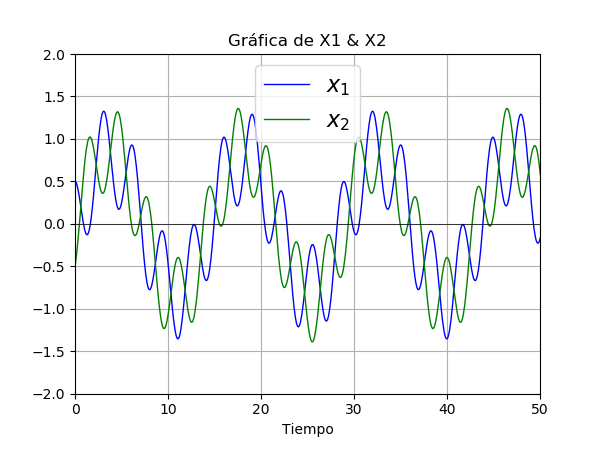
\includegraphics[height=9cm]{Ejem2_3-GrafE}
        \caption{Gráfica del ejemplo 2.3}

        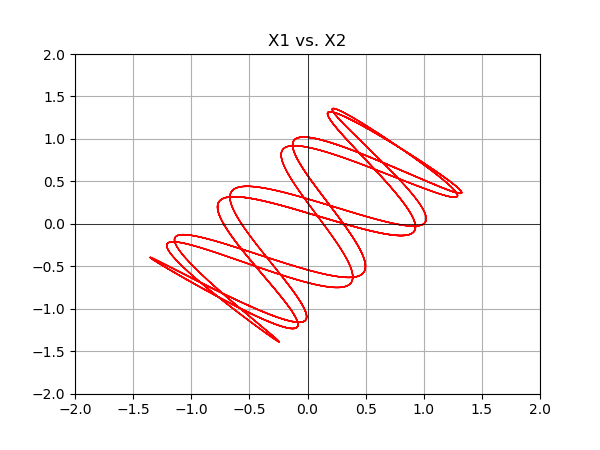
\includegraphics[height=9cm]{Ejem2_3-GrafF}
        \caption{Gráfica del ejemplo 2.3}
        \label{Ejem2.3-GrafF}
    \end{center}
\end{figure}

Finalmente, para el \textbf{ejemplo 2.4} tendremos las Figuras \ref{Ejem2.4-GrafA} a \ref{Ejem2.4-GrafF}.

\begin{figure}[h!]
	\begin{center}
        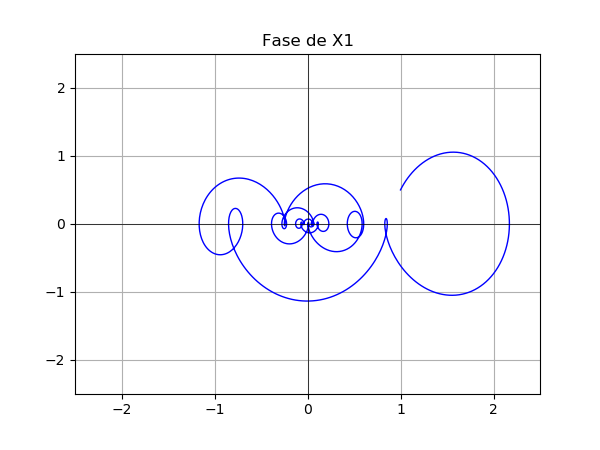
\includegraphics[height=9cm]{Ejem2_4-GrafA}
        \caption{Gráfica del ejemplo 2.4}
        \label{Ejem2.4-GrafA}

        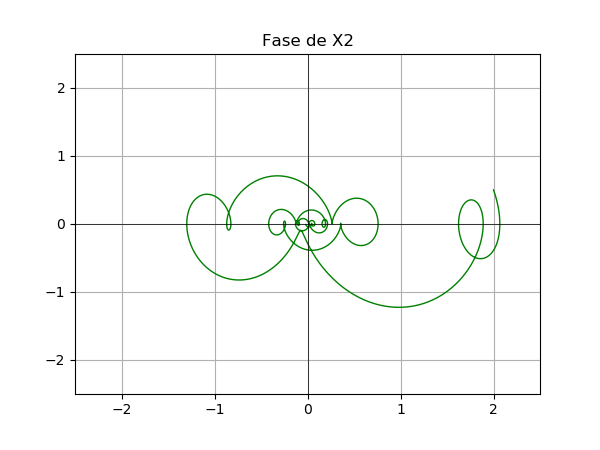
\includegraphics[height=9cm]{Ejem2_4-GrafB}
        \caption{Gráfica del ejemplo 2.4}
    \end{center}
\end{figure}

\begin{figure}[h!]
	\begin{center}
        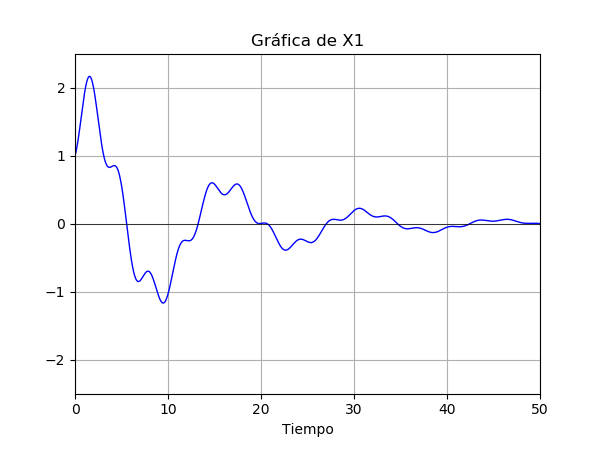
\includegraphics[height=9cm]{Ejem2_4-GrafC}
        \caption{Gráfica del ejemplo 2.4}

    	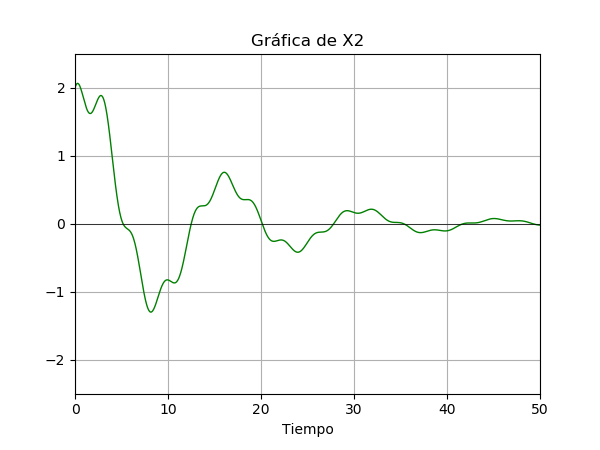
\includegraphics[height=9cm]{Ejem2_4-GrafD}
        \caption{Gráfica del ejemplo 2.4}
    \end{center}
\end{figure}

\begin{figure}[h!]
	\begin{center}
        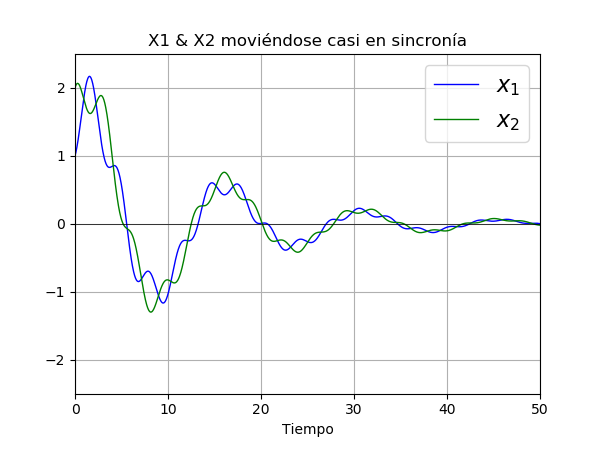
\includegraphics[height=9cm]{Ejem2_4-GrafE}
        \caption{Gráfica del ejemplo 2.4}

        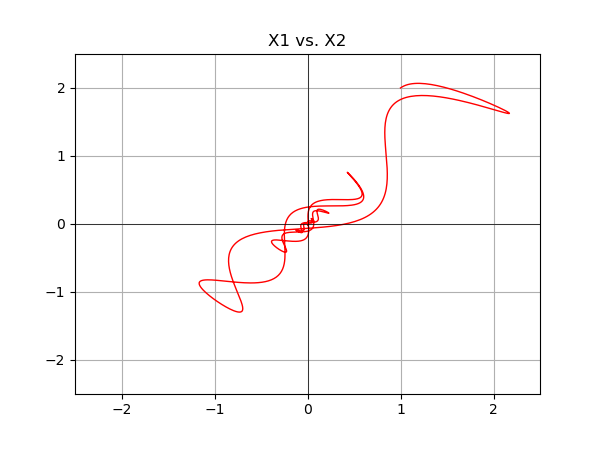
\includegraphics[height=9cm]{Ejem2_4-GrafF}
        \caption{Gráfica del ejemplo 2.4}
        \label{Ejem2.4-GrafF}
    \end{center}
\end{figure}

%\vfill
%\vline
%\space
%\par %\vspace{0.5cm}

\section{Apéndice}
\begin{enumerate}
\item \textbf{¿En general te pareció interesante esta actividad de modelación matemática? ¿Qué te gustó mas? ¿Qué no te gustó?}
\medskip
\\ Me pareció sencilla pues ya habíamos trabajado anteriormente en graficar datos, lo nuevo fue estudiar cómo funciona el código.

\item \textbf{La cantidad de material te pareció ¿bien?, ¿suficiente?, ¿demasiado?}
\medskip
\\ La cantidad de material está bien, no fue demasiado ni muy poco.

\item \textbf{¿Cuál es tu primera impresión de Jupyter Lab?}
\medskip
\\ Me gusta mucho más este aspecto de trabajo a simplemente Jupyter Notebook, me siento un poco más organizado y con mayor libertad al hacer el trabajo de esta forma.

\item \textbf{Respecto al uso de funciones de SciPy, ¿ya habías visto integración numérica en tus cursos anteriores? ¿Cuál es tu experiencia?}
\medskip
\\ Habíamos aplicado integración por métodos numéricos más sin embargo, fueron códigos que nosotros creamos y no eran parecidos a los que se aplicaron en esta actividad.

\item \textbf{El tema de sistema de masas acopladas con resortes, ¿ya lo habías resuelto en tu curso de Mecánica 2?}  
\medskip
\\ No habíamos resuelto las ecuaciones ni tampoco recuerdo haberlas desarrollado tanto pero de igual forma teníamos la idea de cómo trabajarlas.

\item \textbf{¿Qué le quitarías o agregarías a esta actividad para hacerla más interesante y divertida?}
\medskip
\\ Quizás eliminaría o por lo menos reduciría aquello del resumen de los primeros dos capítulos de la lectura.

\end{enumerate}

\end{document}